\documentclass{article}

\usepackage{graphicx}
\usepackage[utf8]{inputenc}
\usepackage[T1]{fontenc}
\usepackage[francais]{babel}
\usepackage{hyperref}
\usepackage{amsmath,amsfonts,amssymb}
\usepackage{Tkz-Tab}
\usepackage{wrapfig}
\usepackage{verbatim}
\usepackage{array}

\begin{document}

\title{Gestion de flux dans le réseau
	\smallbreak
	TD n\degre5
	\smallbreak
	Modélisation mathématique
	\smallbreak
	Q4}
\author{Sibylle Roux \and Juliette Arazo \and Nicolas Le Gallo \and Tanguy Thomas}

\maketitle

\newpage

\tableofcontents

\newpage

\section{Essaies randoms}

\subsection{}

\section{Etude mathématique de la loi tente}

\subsection{Densité}

\subsubsection{Fonction}

$$
f(x)=\left\{
	\begin{array}{ll}
		1-|x| & \mbox{si} -1<=x<=1\\
		0 & \mbox{sinon}
	\end{array}
\right.
$$

\subsubsection{Représentation graphique}
\begin{center}
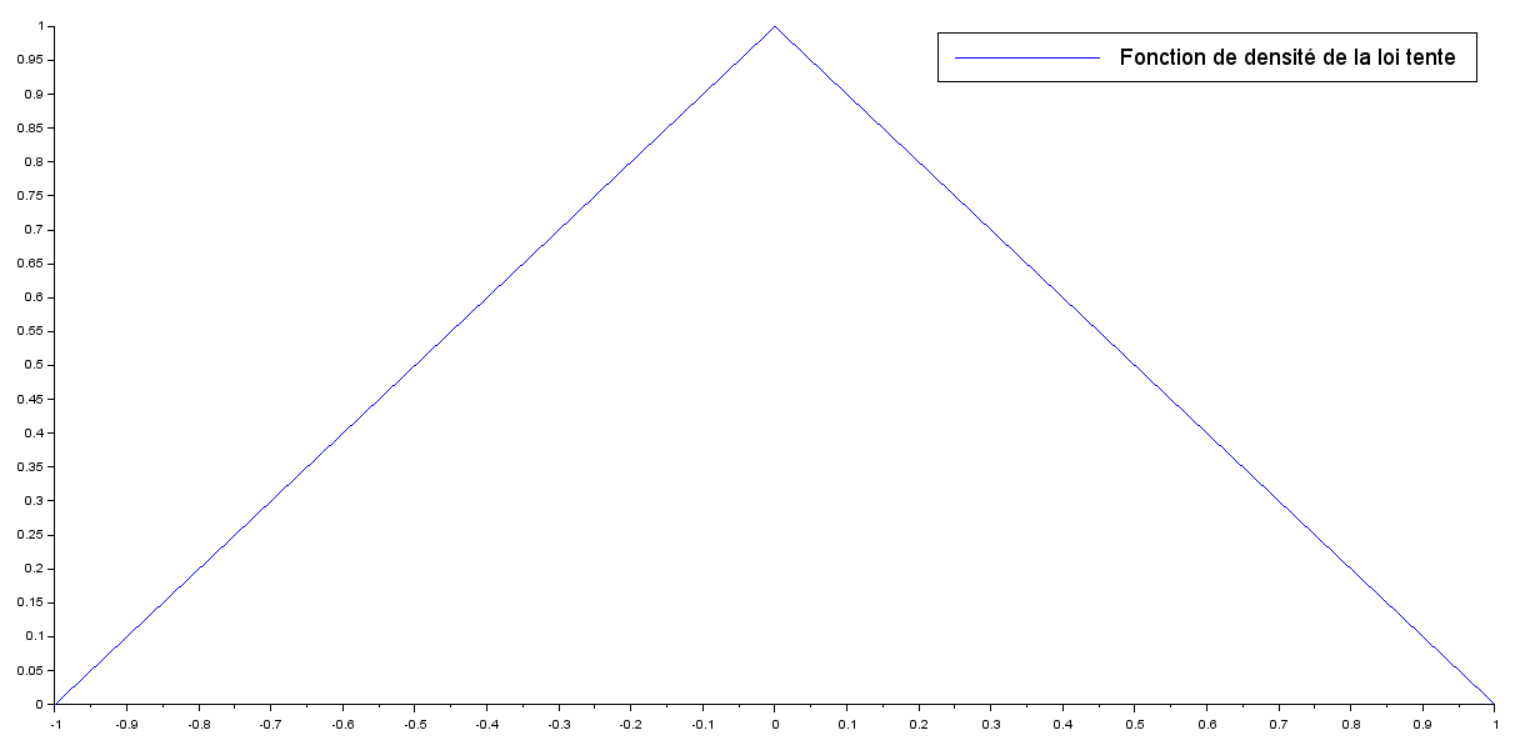
\includegraphics[width=425px]{img/tente.png}
\end{center}
\paragraph{}

\subsection{Fonction de répartition}

\subsubsection{Fonction}
%TODO

\subsubsection{Représentation graphique}
\begin{center}
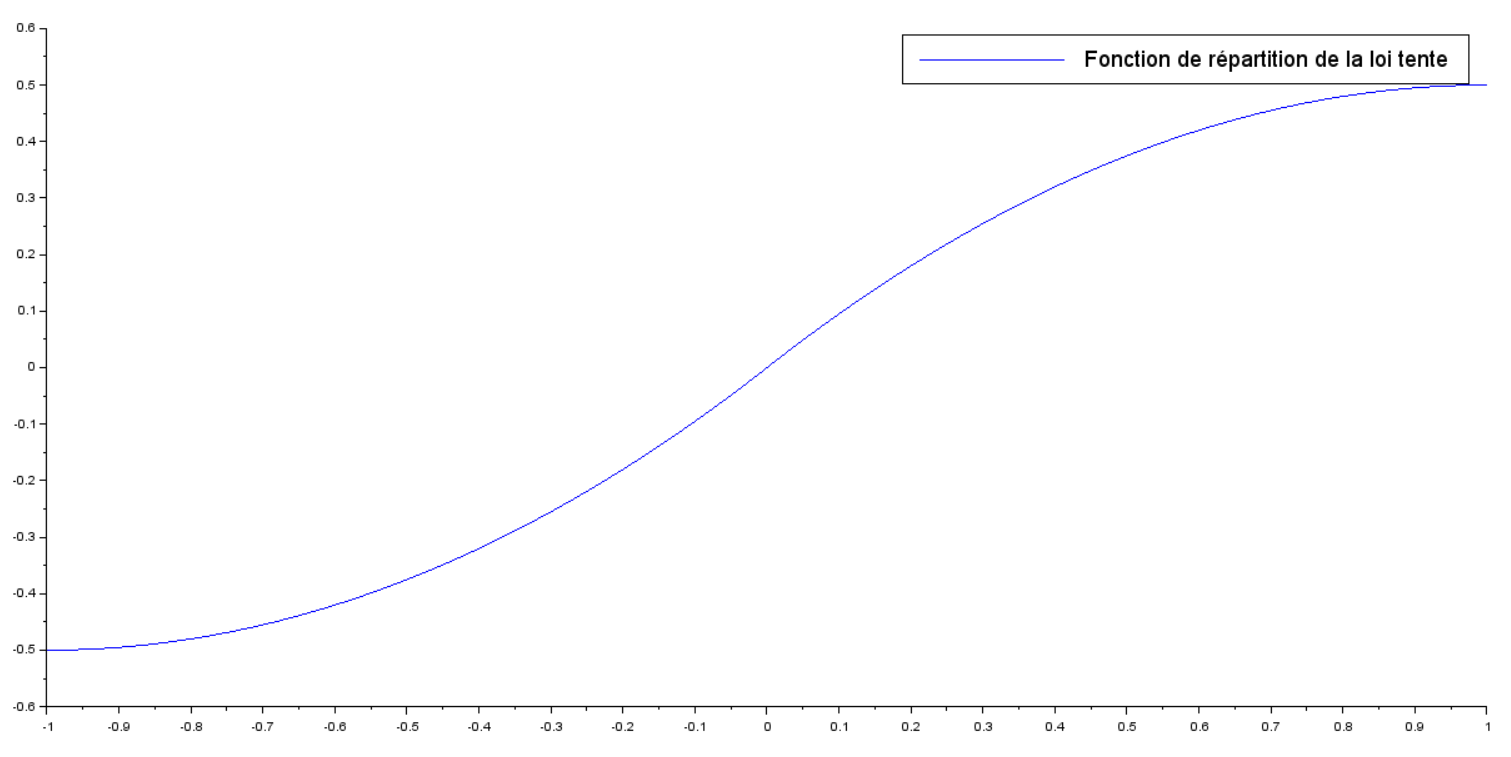
\includegraphics[width=425px]{img/tente_repartition.png}
\end{center}
\paragraph{}

\subsection{Inverse}

\part{Conclusion}
\paragraph{}

\newpage
\appendix

\section{}

\subsection{}

\subsubsection{}
\begin{verbatim}
\end{verbatim}

%----------------------------------


\end{document}